
\chapter{Evaluation}
\subsection{Evaluating network performance on training/test split of OSM Tiles}
We begin with an evaluation of the MapNet network trained on map tiles obtained from the Oxford Area. The GPS bounds delineating the area of our map tiles are the following:

(lat\_min, lon\_min) = (-1.272869110107422, 51.75041438844966)\\
(lat\_max, lon\_max) = (-1.2330436706542969, 51.76868973964186)

\myfig{thesis/test_map}%% filename
{scale=0.1}%% width/height
{Area to train our localization on map tiles. Taken from OSM.}%% caption
{OpenStreetMap training area}%% optional (short) caption for list of figures
{Ev1.0}

As described in our methodology section, we sample from this map area overlapping map tiles at zoom level 19. After converting these tiles into binary images which depict car point-of-view building contours. Our network is trained on pairs of these tiles and their offset from a reference tile (approx. 16800 tiles).

\myfig{thesis/test_map_gps_sample}%% filename
{scale=0.4}%% width/height
{Red dots indicate locations where we sample tiles. For visibility purposes, we only show samples at fixed intervals. Taken from OSM.}%% caption
{OpenStreetMap tile samples}%% optional (short) caption for list of figures
{Ev1.1}

We uniformly sample every 8th tile from our original dataset, and include it in our test dataset for evaluation (approx. 2100 tiles). Note that the test set follows the same trajectory as the training tile sequence. After training for 200 epochs, we predict the positions of our test tiles. 
\\
\myfig{thesis/test_traj.png}%% filename
{scale=0.4}%% width/height
{Predictions of MapNet on test tiles sampled from the training tile trajectory. Red Dots - Prediction, Green - Ground Truth. Blue lines - prediction to ground truth mappings}%% caption
{Test trajectory prediction}%% optional (short) caption for list of figures
{Ev1.2}

We note first that a majority of our predictions are close to the ground truth, with a few predictions being quite noisy (note that several noisy predictions tend toward almost the same (wrong) tile). The figure below showcases more precise statistics, i.e. a distribution of tiles over localization error in tile-widths.

\myfig{thesis/tile_osm_hist.png}%% filename
{scale=0.25}%% width/height
{Distribution of test tile localization error}%% caption
{Test tile prediction histogram}%% optional (short) caption for list of figures
{Ev1.3}

As we can see, more than 75\% of the test tiles lie within 5 error widths of the ground truth tile, with more than 50\% within 2 tile widths. 

\subsubsection{Effects of Rotation, Translation and Scaling of query tile}
While creating the query tile from the pointcloud of the scene, we take care to ensure that our query tile is oriented in the True North direction (which is the direction of the default orientation of OpenStreetMap tiles) and to ensure that the distance encoded by each pixel roughly matches the resolution of the respective OSM tile.

We prove the necessity for this procedure by showing the changes in accuracy of localization when varying the orientation, scale and translation of the query tiles.

\subsubsection{Rotation}
We check the error profile for each tile, for orientations at an interval of 30 degrees between them. We note from the plots below that predictions get significantly noisier as we rotate the tiles away from their true orientation. 

\begin{figure}
	\begin{longtable}{cc}
		\subfloat[No modification]{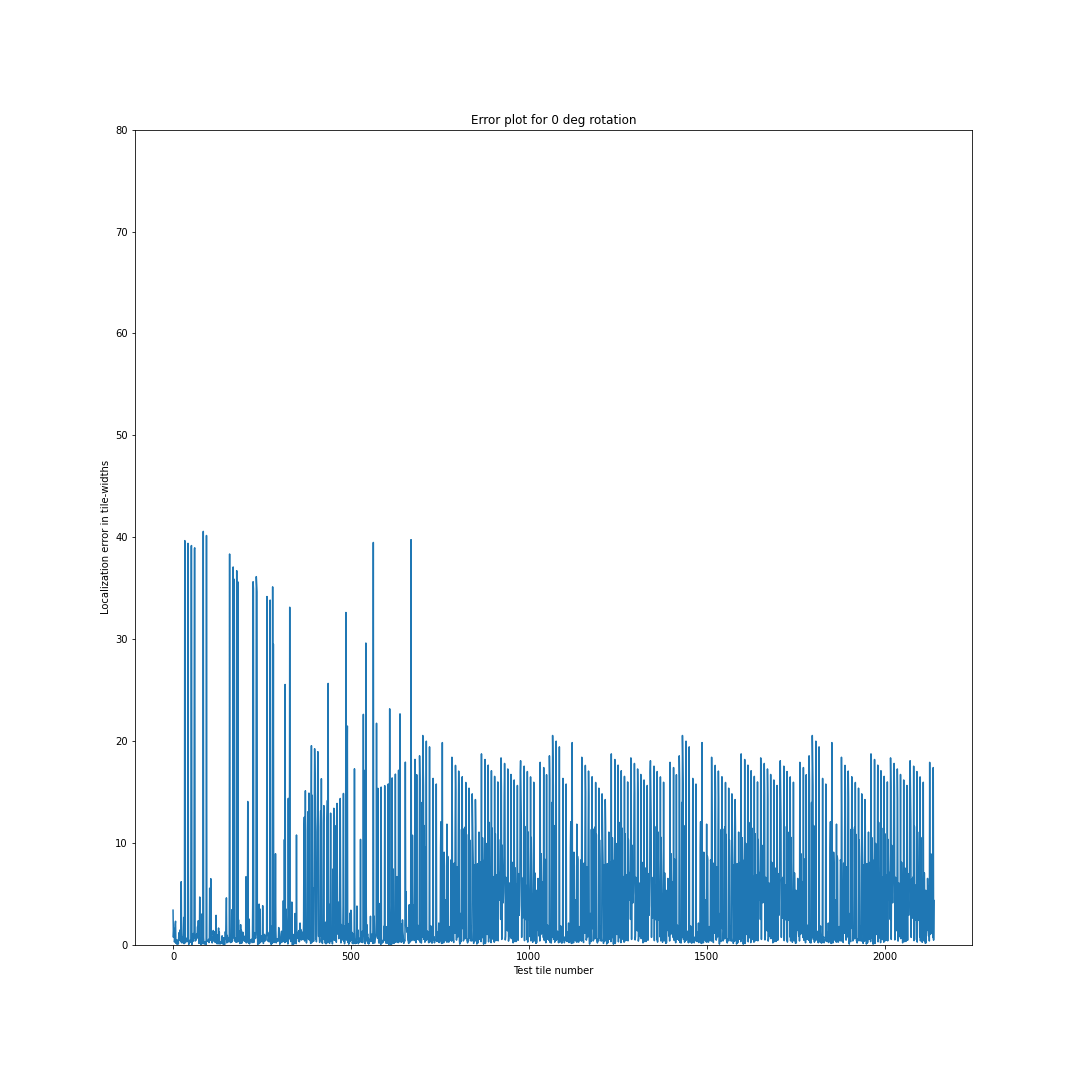
\includegraphics[width = 2.0in]{figures/thesis/plt_folder/rotate_error_0}} &
		\subfloat[No modification - error distribution]{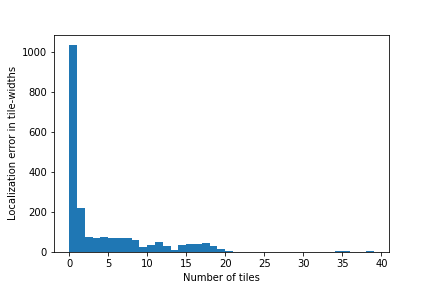
\includegraphics[width = 2.0in]{figures/thesis/plt_folder/rotate_hist_0}}
	\end{longtable}
\caption{Predictions on unmodified tiles. Note that most predictions lie within 3 tile widths' error, with the rest tapering off to higher errors.}
\end{figure}

\begin{figure}
	\begin{longtable}{cc}
		\subfloat[30 degrees]{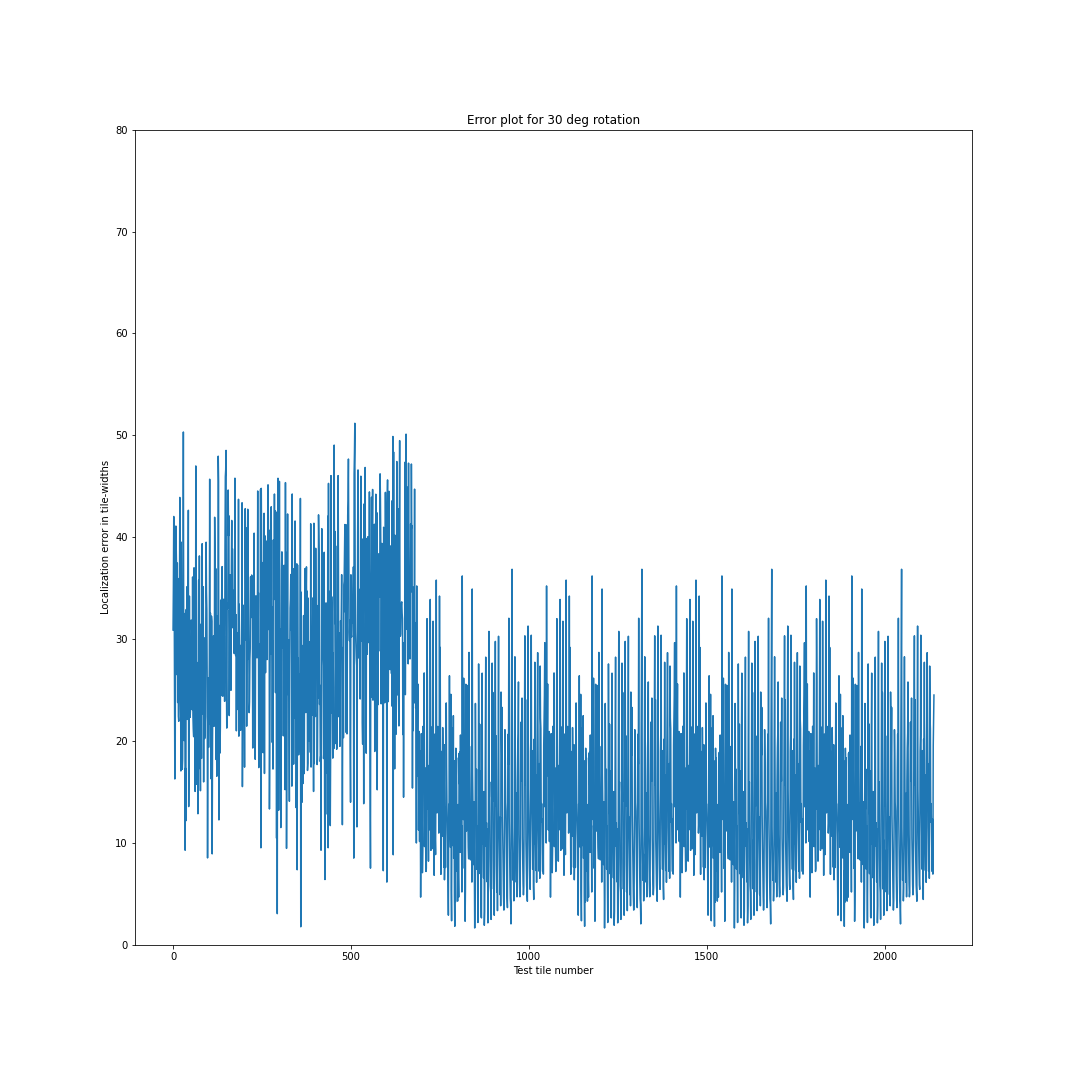
\includegraphics[width = 1.5in]{figures/thesis/plt_folder/rotate_error_30}} &
		\subfloat[30 degrees error distribution]{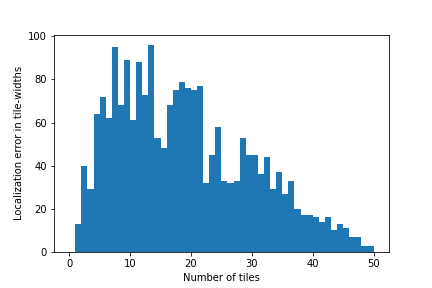
\includegraphics[width = 1.5in]{figures/thesis/plt_folder/rotate_hist_30}}\\
		\subfloat[60 degrees]{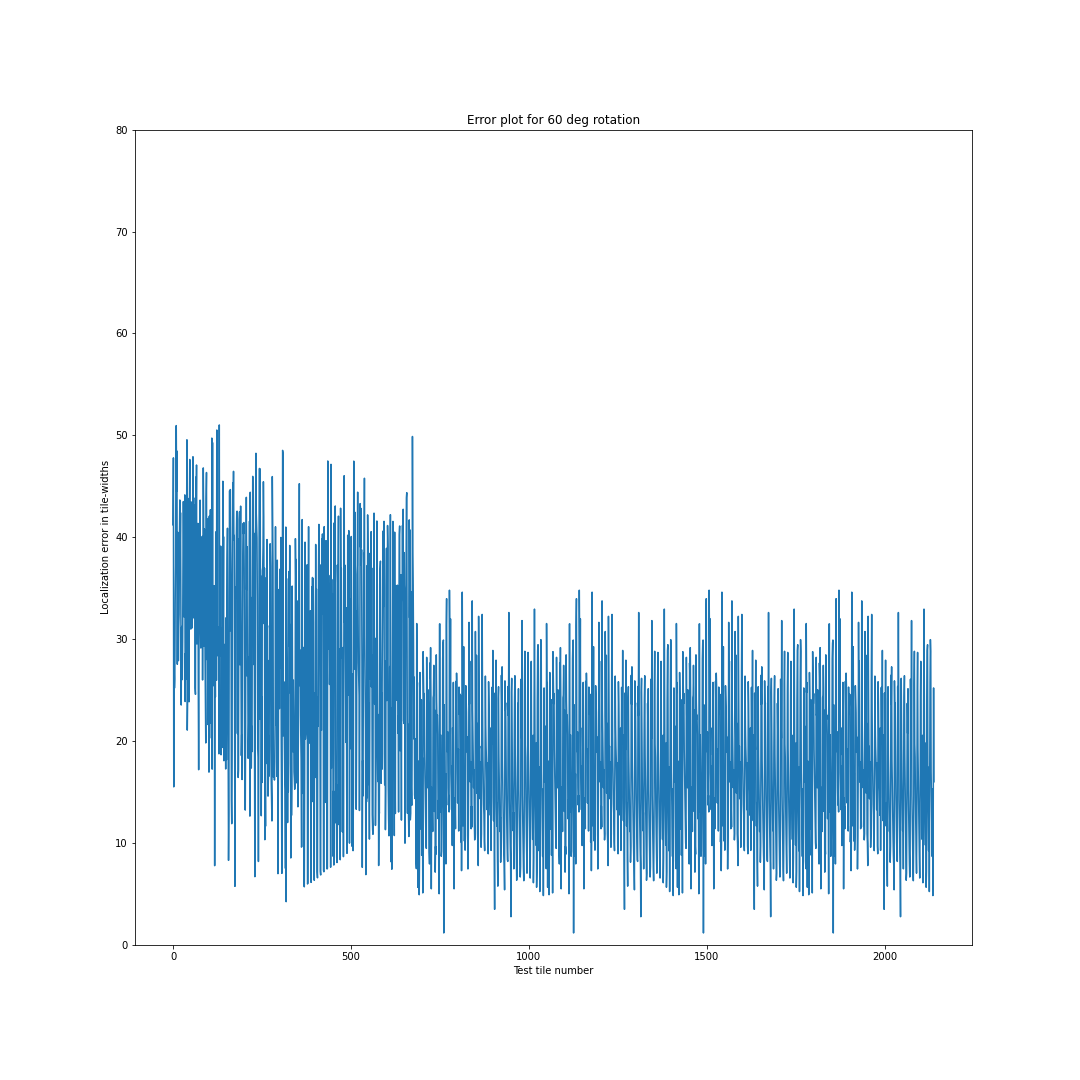
\includegraphics[width = 1.5in]{figures/thesis/plt_folder/rotate_error_60}} &
		\subfloat[60 degrees error distribution]{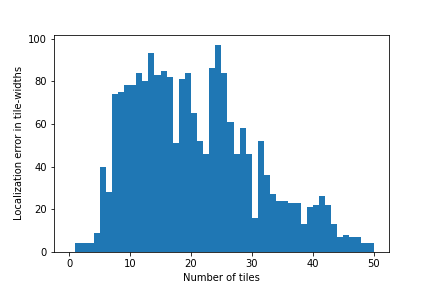
\includegraphics[width = 1.5in]{figures/thesis/plt_folder/rotate_hist_60}}\\
		\subfloat[90 degrees]{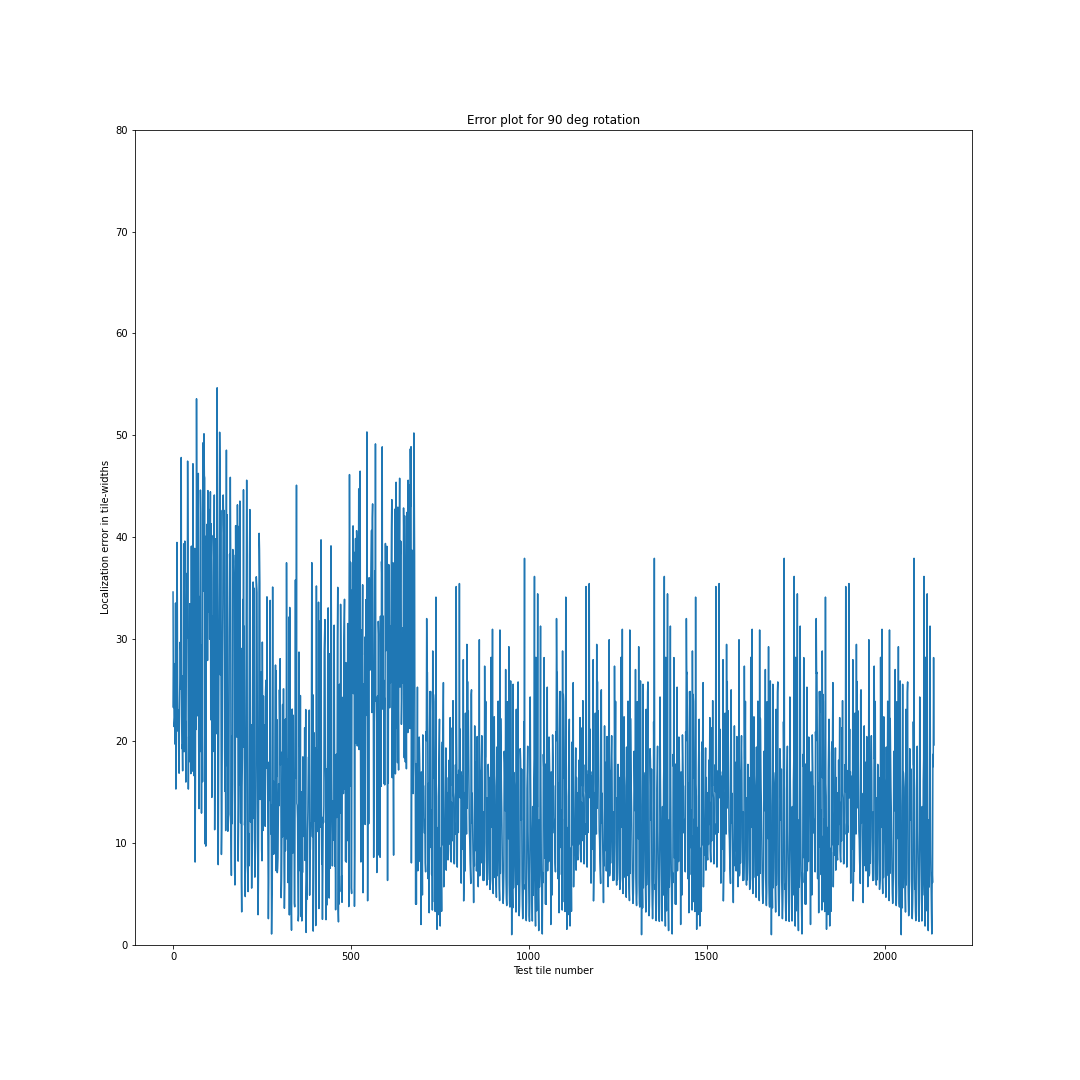
\includegraphics[width = 1.5in]{figures/thesis/plt_folder/rotate_error_90}} &
		\subfloat[90 degrees error distribution]{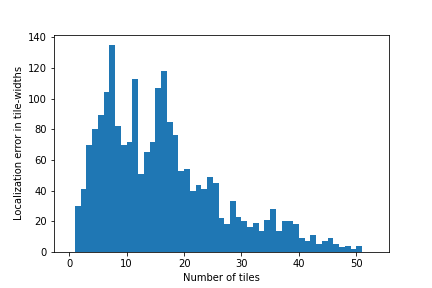
\includegraphics[width = 1.5in]{figures/thesis/plt_folder/rotate_hist_90}} \\
		\subfloat[120 degrees]{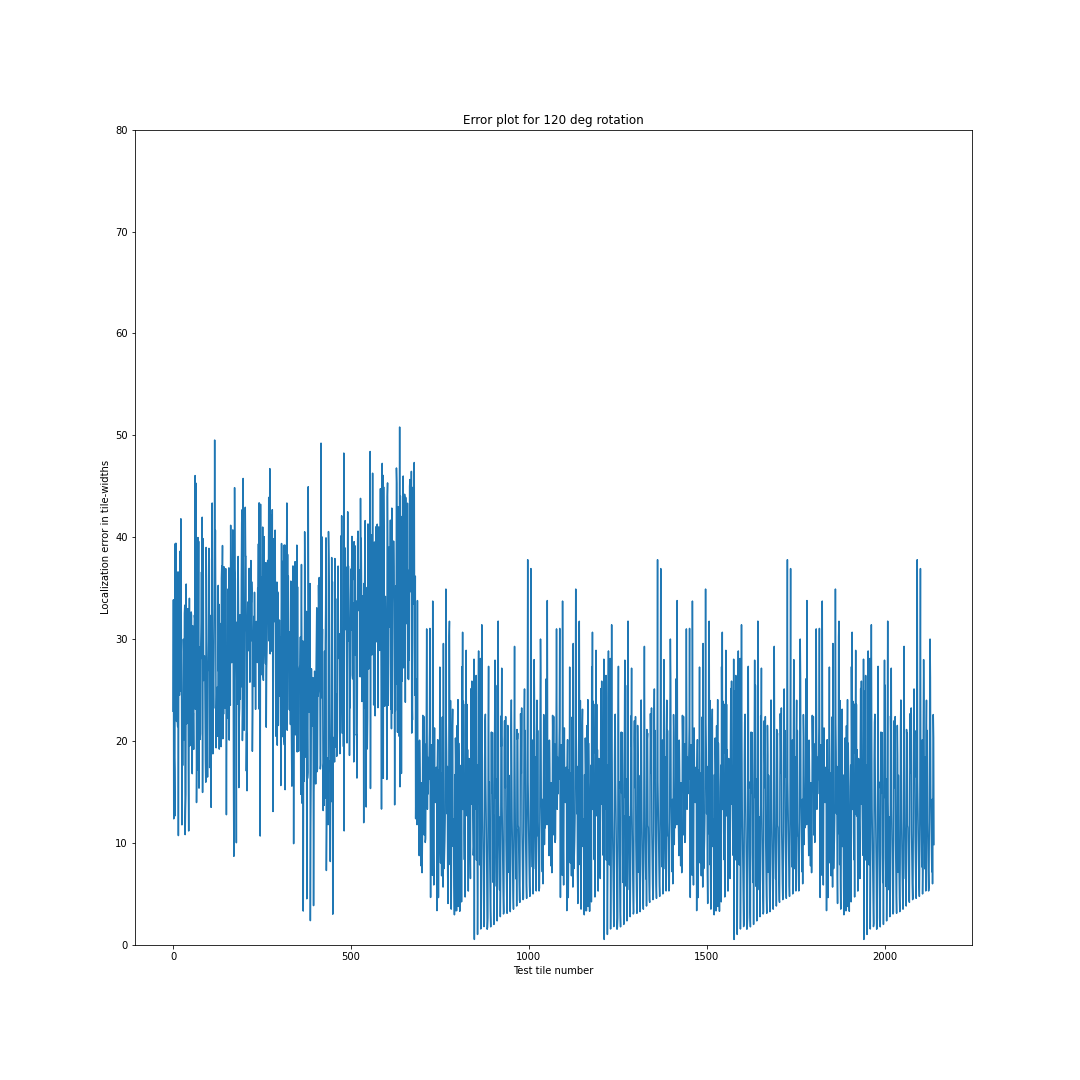
\includegraphics[width = 1.5in]{figures/thesis/plt_folder/rotate_error_120}}&
		\subfloat[120 degrees error distribution]{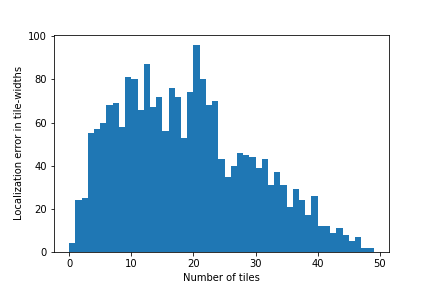
\includegraphics[width = 1.5in]{figures/thesis/plt_folder/rotate_hist_120}}\\
	\end{longtable}
\end{figure}
		
	\begin{figure}
		\begin{longtable}{cc}	
		\subfloat[150 degrees]{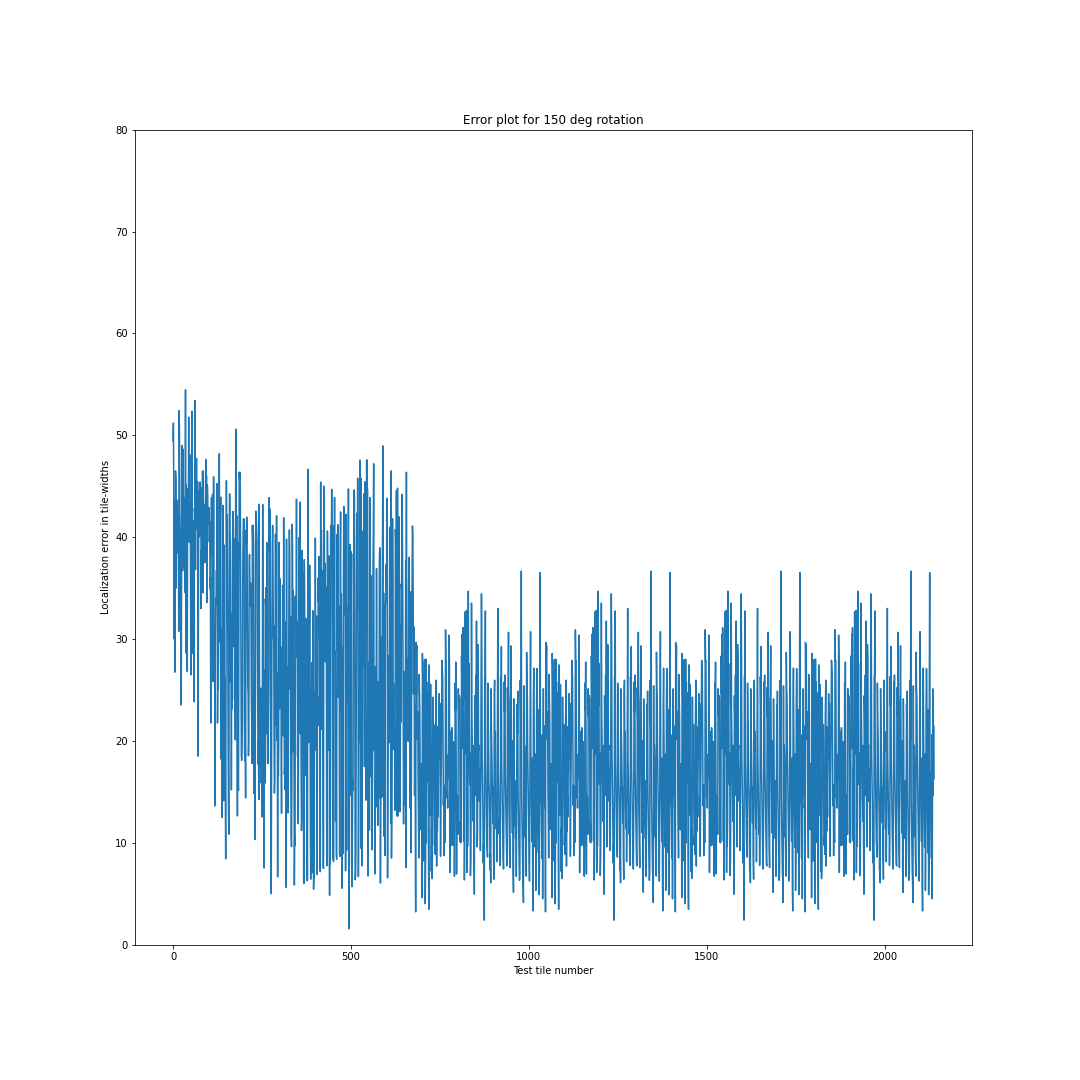
\includegraphics[width = 1.5in]{figures/thesis/plt_folder/rotate_error_150}} &
		\subfloat[150 degrees error distribution]{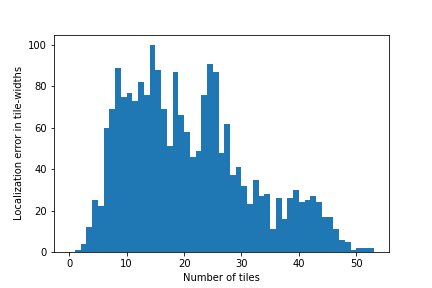
\includegraphics[width = 1.5in]{figures/thesis/plt_folder/rotate_hist_150}}\\
		\subfloat[180 degrees]{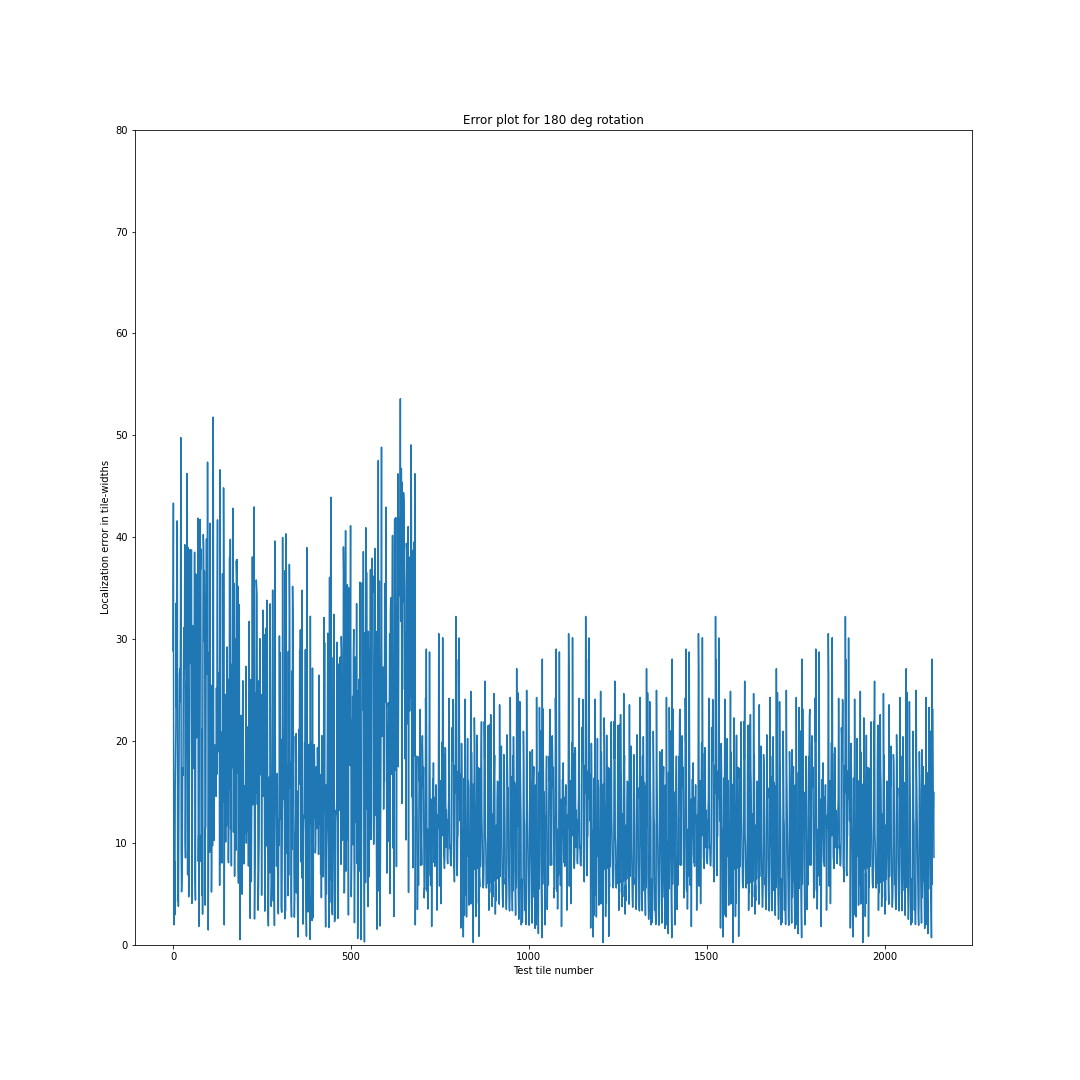
\includegraphics[width = 1.5in]{figures/thesis/plt_folder/rotate_error_180}} &
		\subfloat[180 degrees error distribution]{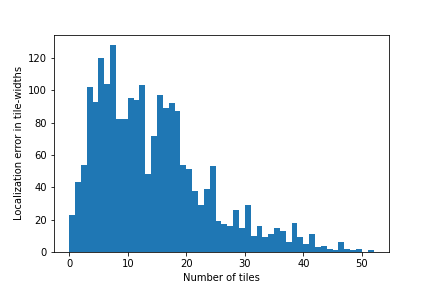
\includegraphics[width = 1.5in]{figures/thesis/plt_folder/rotate_hist_180}}\\
		\subfloat[210 degrees]{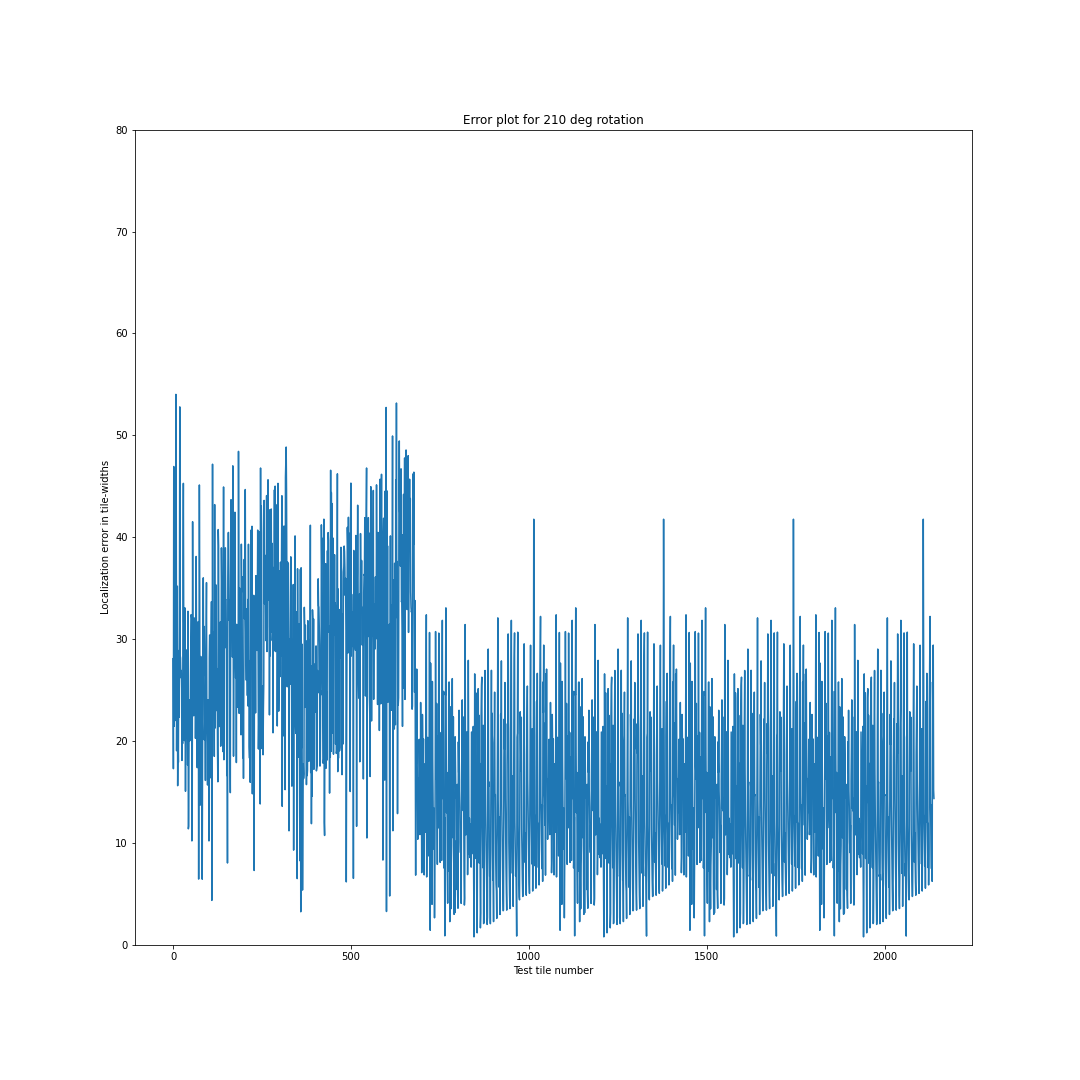
\includegraphics[width = 1.5in]{figures/thesis/plt_folder/rotate_error_210}} &
		\subfloat[210 degrees error distribution]{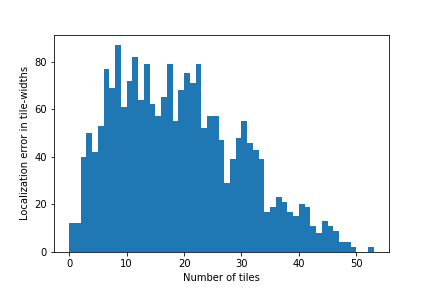
\includegraphics[width = 1.5in]{figures/thesis/plt_folder/rotate_hist_210}}\\
		\subfloat[240 degrees]{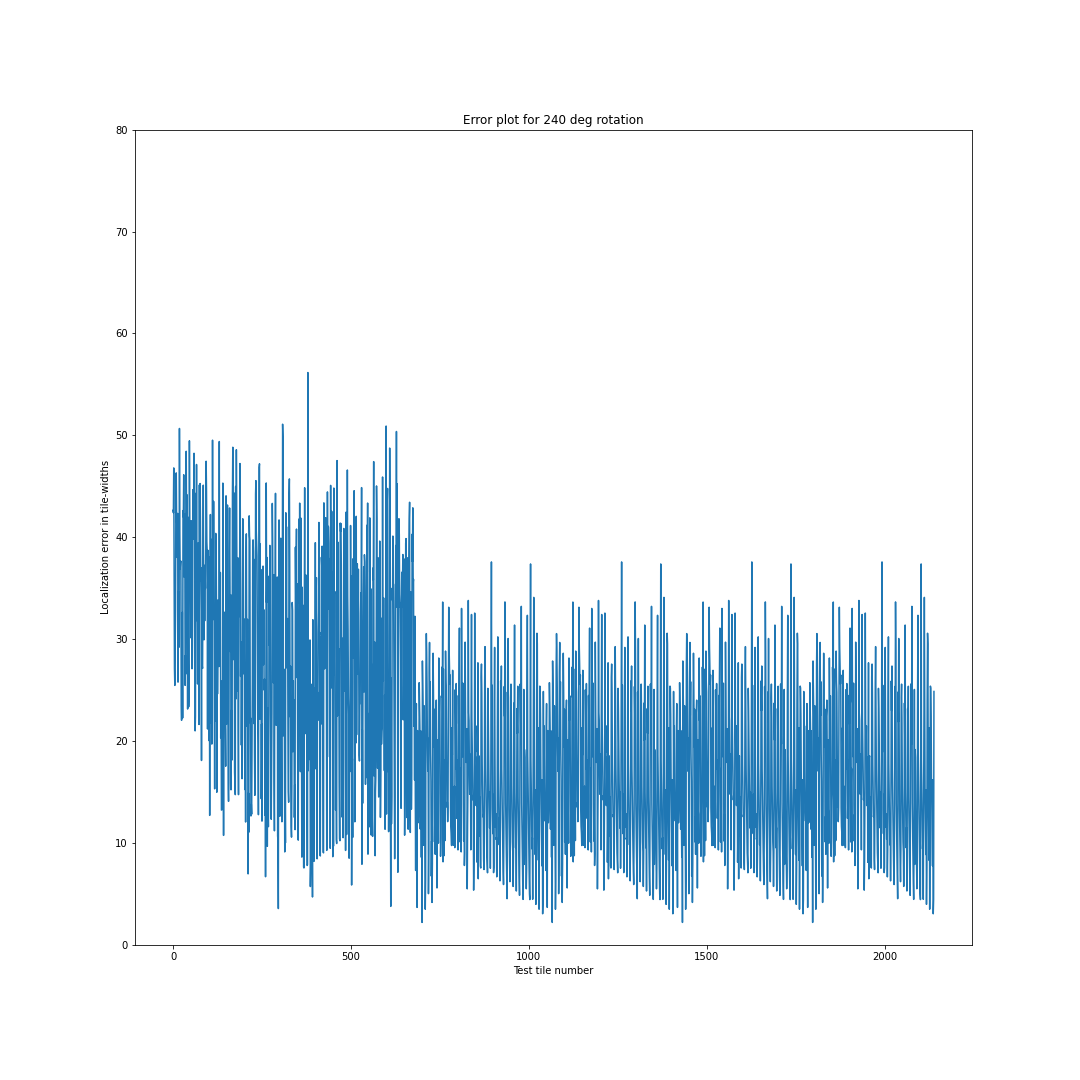
\includegraphics[width = 1.5in]{figures/thesis/plt_folder/rotate_error_240}}&
		\subfloat[240 degrees error distribution]{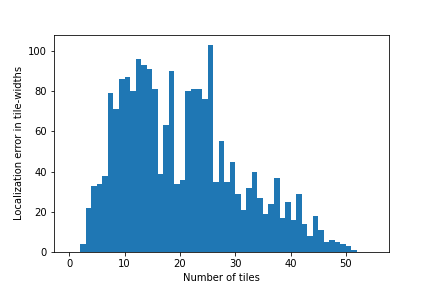
\includegraphics[width = 1.5in]{figures/thesis/plt_folder/rotate_hist_240}}
	\end{longtable}
\end{figure}

	\begin{figure}
	\begin{longtable}{cc}
		\subfloat[270 degrees]{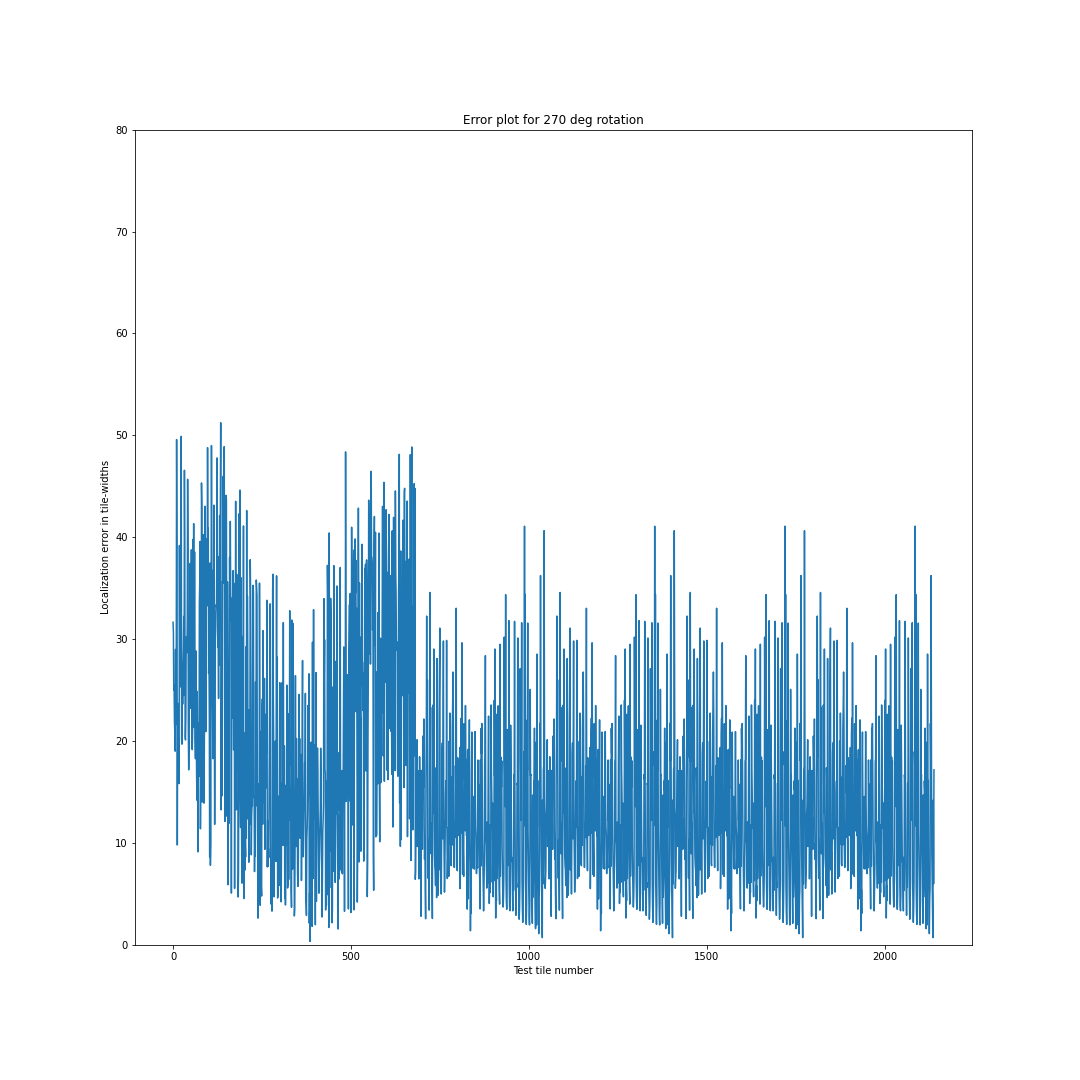
\includegraphics[width = 1.5in]{figures/thesis/plt_folder/rotate_error_270}} &
		\subfloat[270 degrees error distribution]{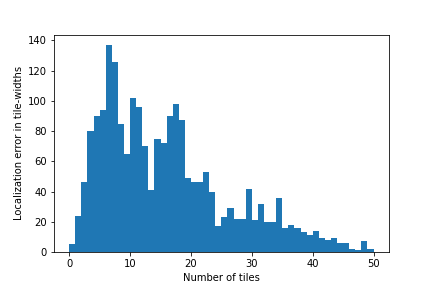
\includegraphics[width = 1.5in]{figures/thesis/plt_folder/rotate_hist_270}}\\
		\subfloat[300 degrees]{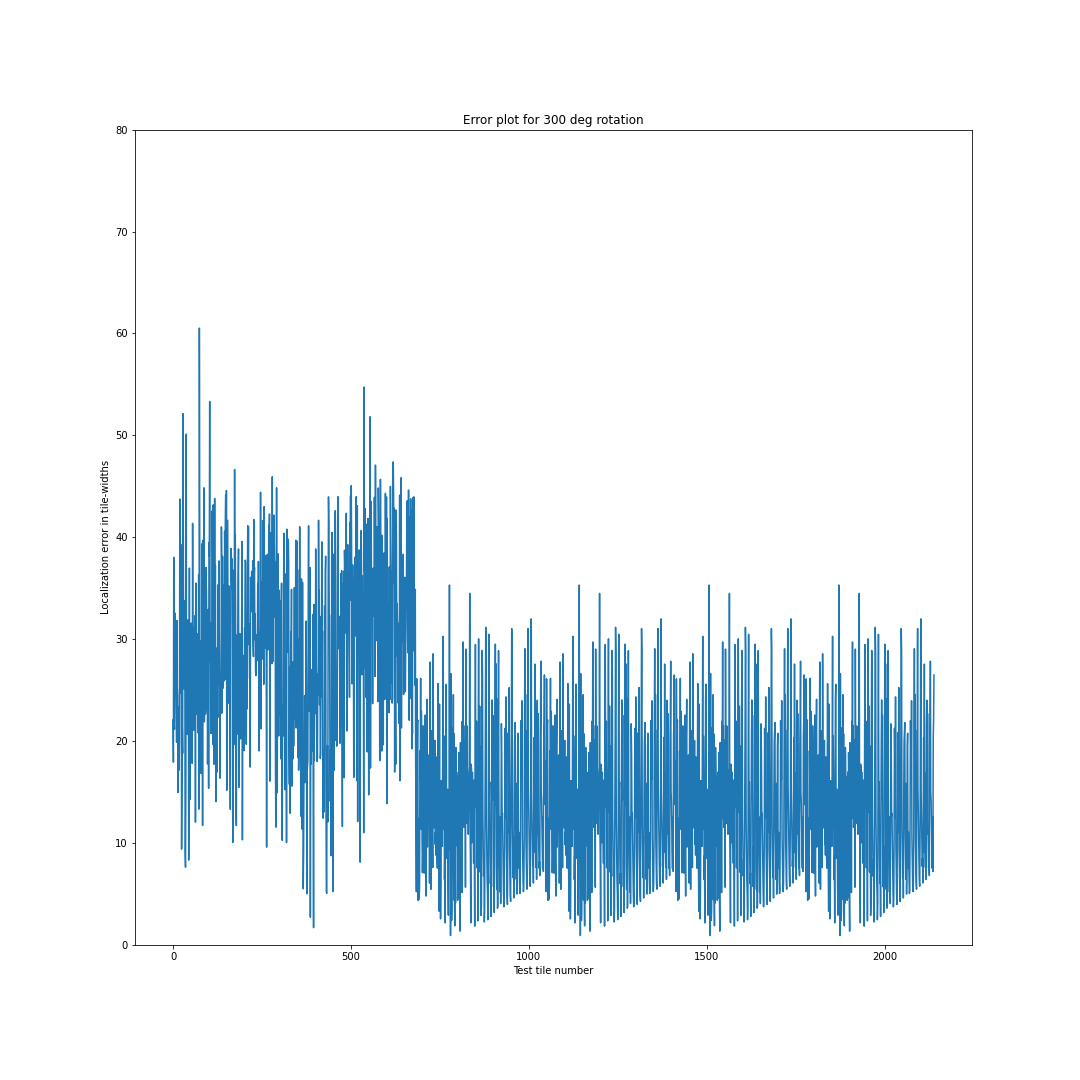
\includegraphics[width = 1.5in]{figures/thesis/plt_folder/rotate_error_300}} &
		\subfloat[300 degrees error distribution]{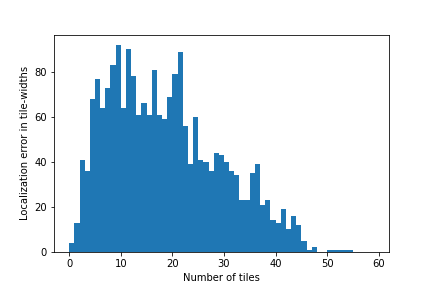
\includegraphics[width = 1.5in]{figures/thesis/plt_folder/rotate_hist_300}}\\
		\subfloat[330 degrees]{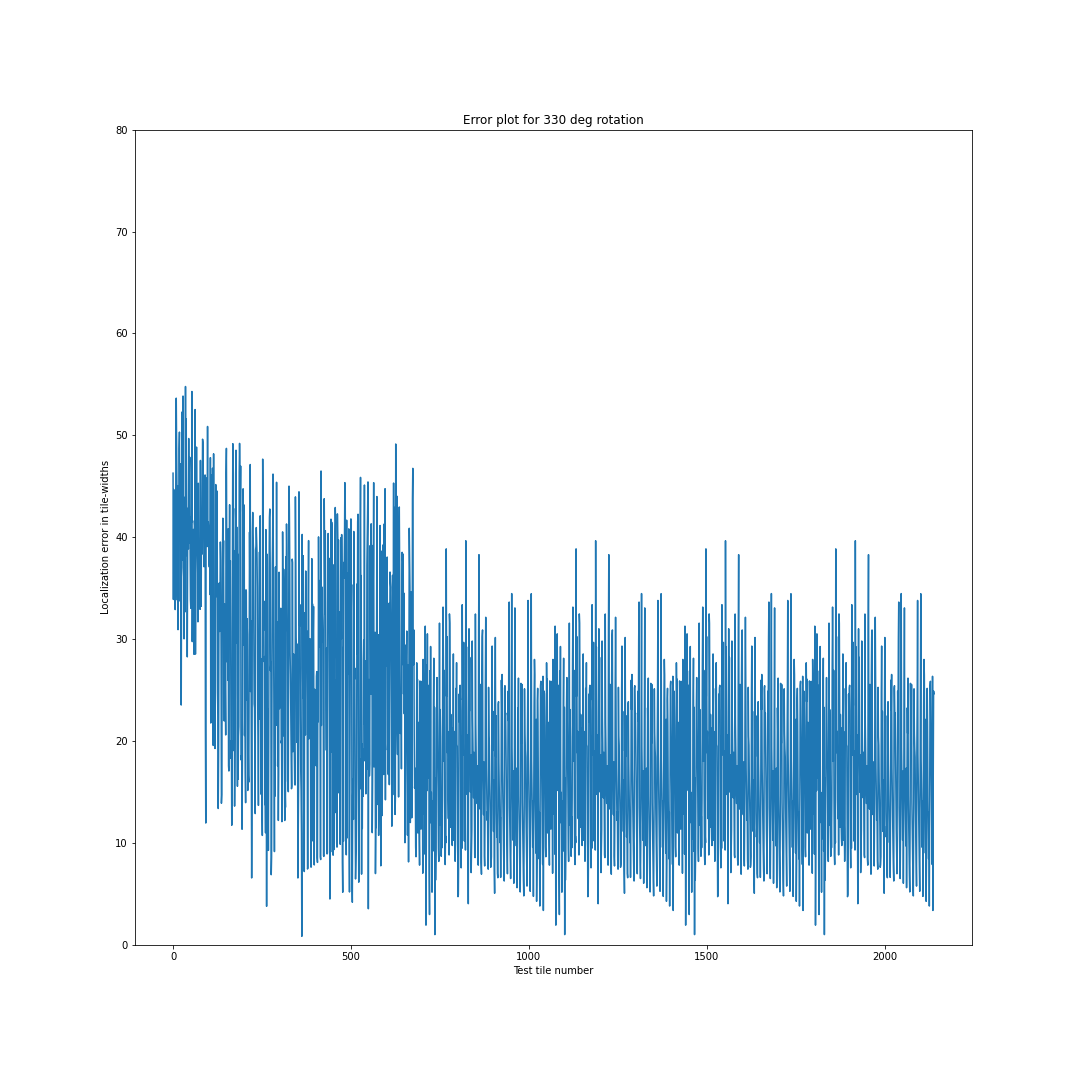
\includegraphics[width = 1.5in]{figures/thesis/plt_folder/rotate_error_330}}&
		\subfloat[330 degrees error distribution]{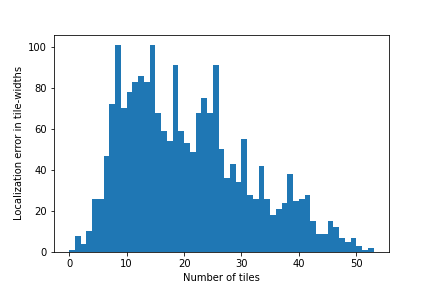
\includegraphics[width = 1.5in]{figures/thesis/plt_folder/rotate_hist_330}}
	\end{longtable}
	\caption{Effect of rotation on localization. We check the error for rotation steps of 30 degrees for the entire dataset, and show that as deviations from the actual orientation yields higher errors.}
\end{figure}

\pagebreak 
\subsubsection{Scaling}
Similarly, we vary the scale of the query tiles and check the prediction error statistics. The error plots below show clearly that the closer we get to the original scale, the lower the likelihood of an erroneous prediction. 

\begin{figure}
	\begin{longtable}{cc}
		\centering
		\subfloat[0.3 scaling]{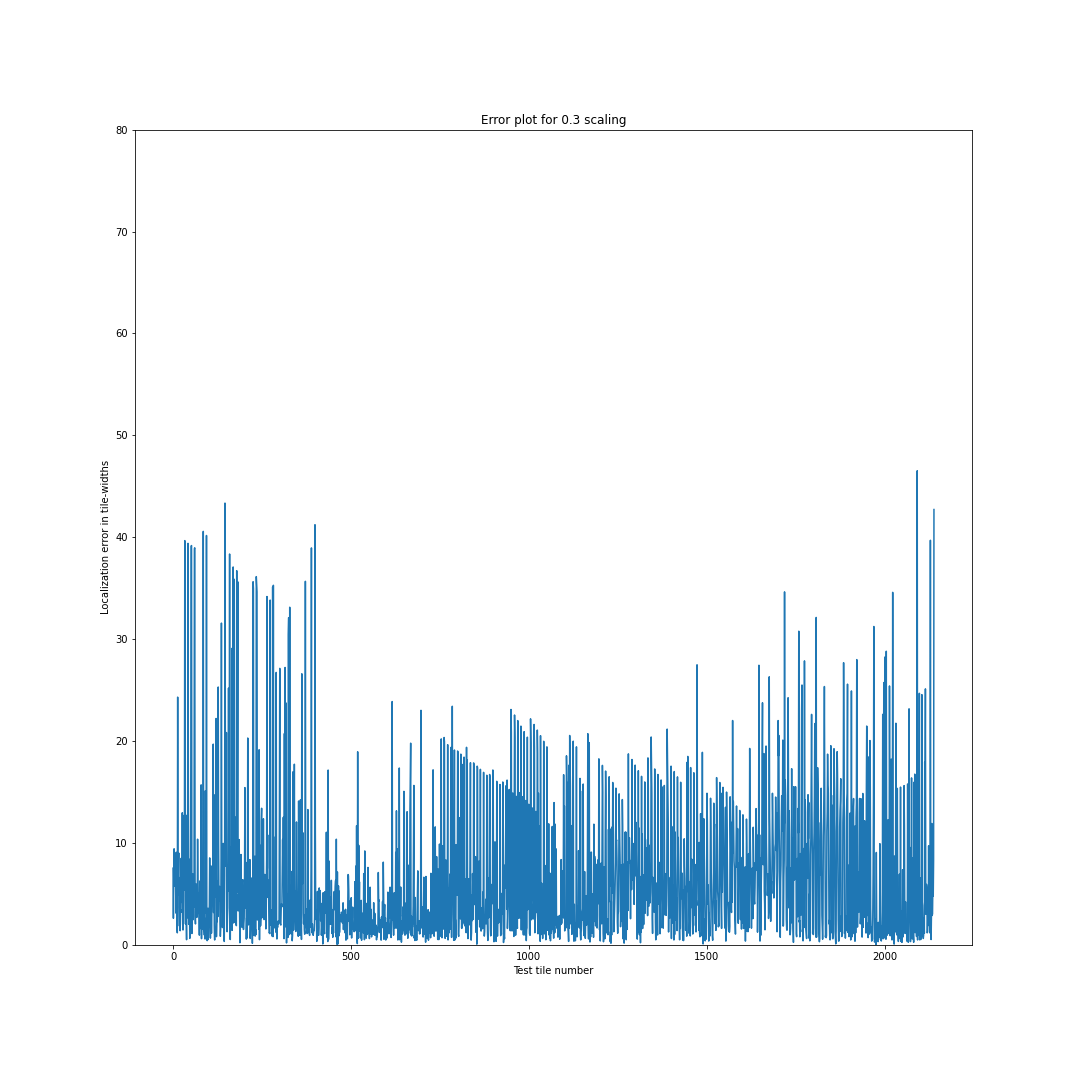
\includegraphics[width = 1.5in]{figures/thesis/plt_folder/scale_error_0.3}} &
		\subfloat[0.3 scaling error distribution]{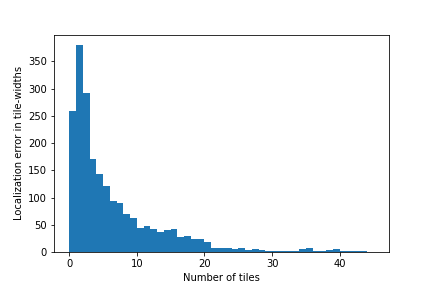
\includegraphics[width = 1.5in]{figures/thesis/plt_folder/scale_hist_0.3}}\\
		\subfloat[0.7 scaling]{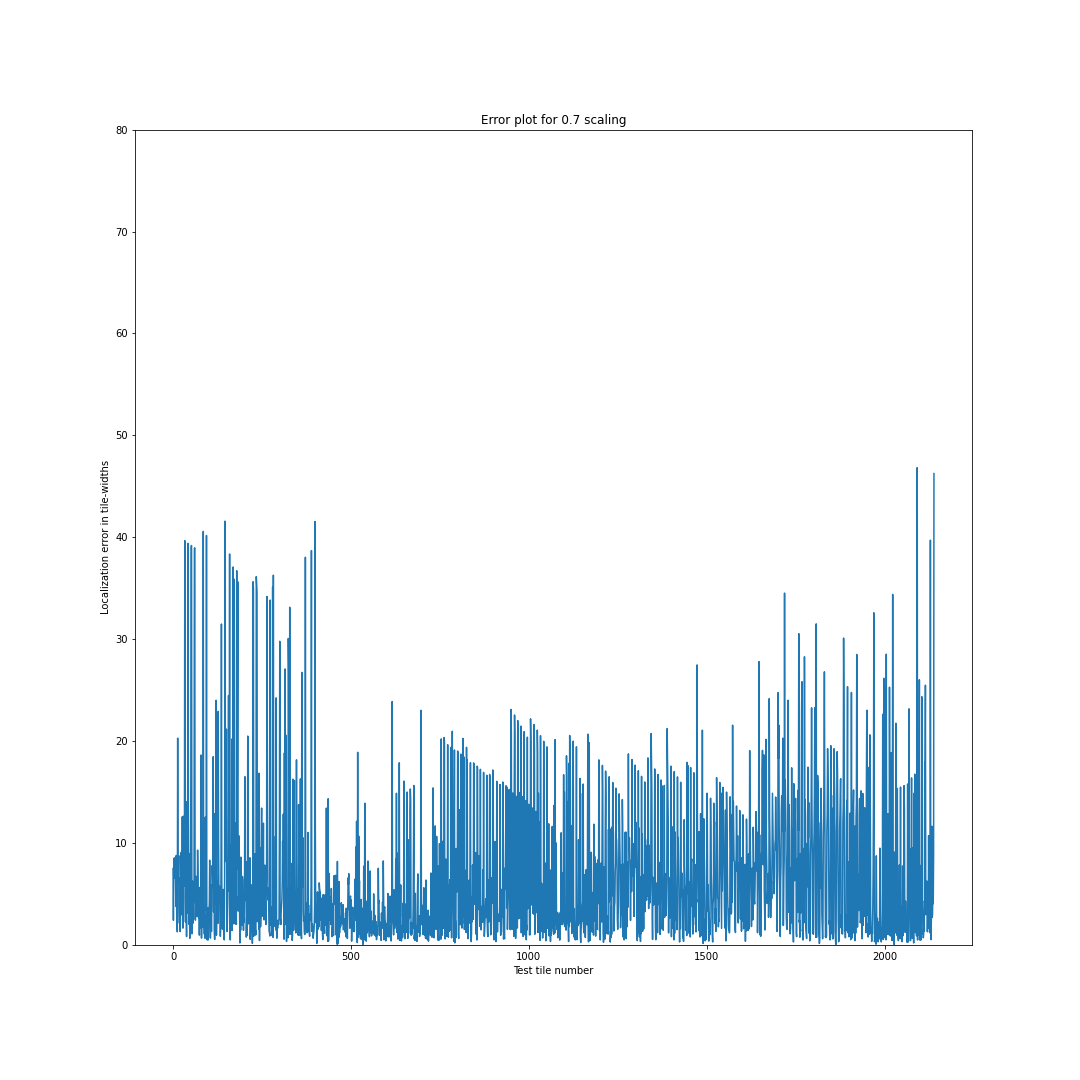
\includegraphics[width = 1.5in]{figures/thesis/plt_folder/scale_error_0.7}} &
		\subfloat[0.7 scalings error distribution]{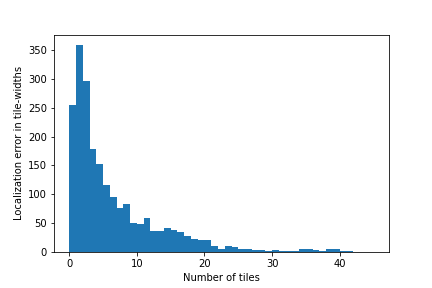
\includegraphics[width = 1.5in]{figures/thesis/plt_folder/scale_hist_0.7}}\\
		\subfloat[1.1 scaling]{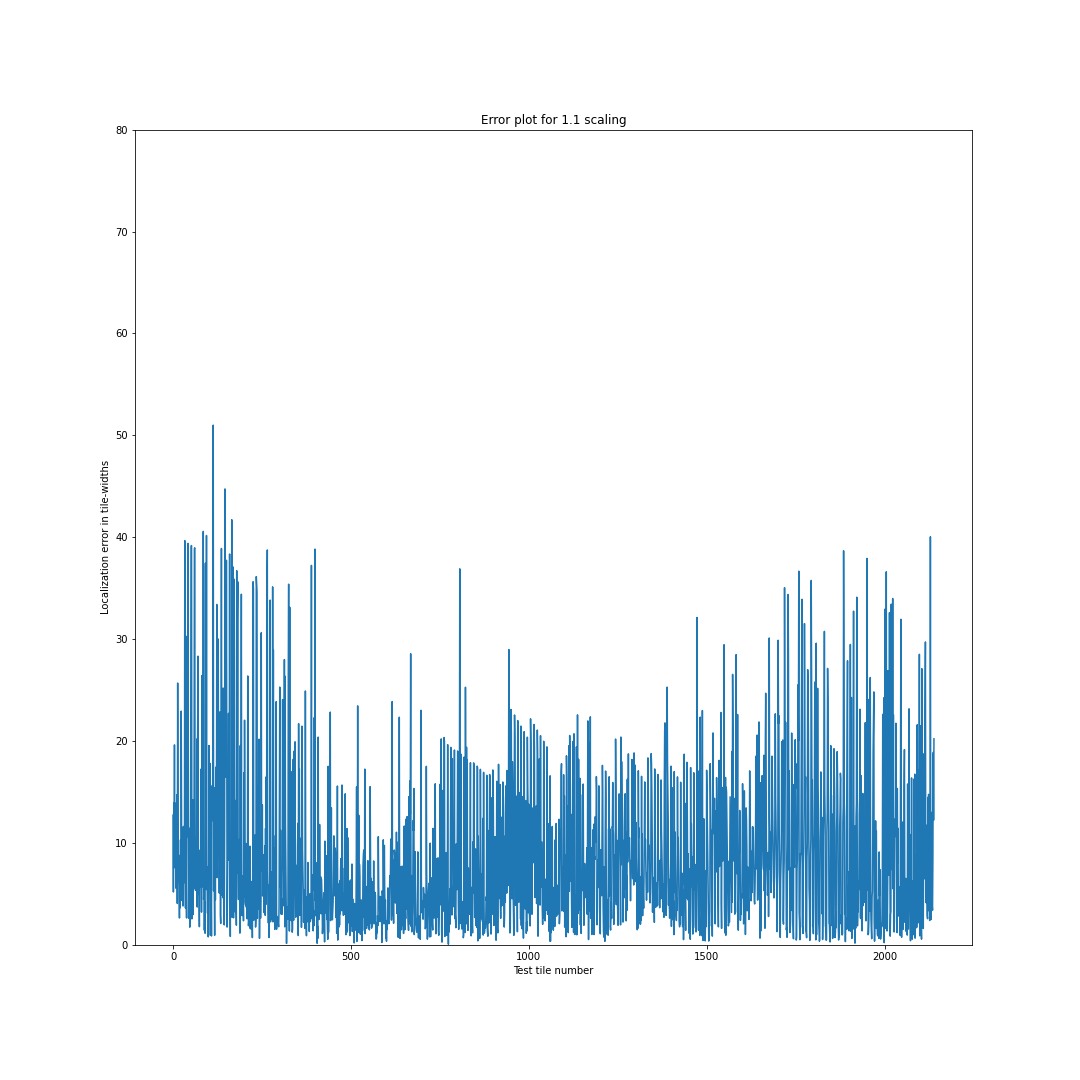
\includegraphics[width = 1.5in]{figures/thesis/plt_folder/scale_error_1.1}} &
		\subfloat[1.1 scaling error distribution]{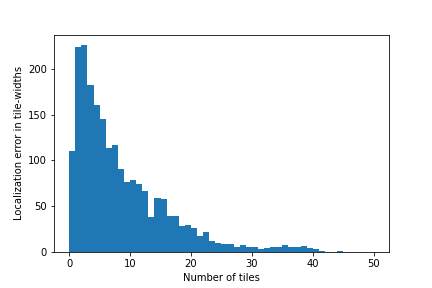
\includegraphics[width = 1.5in]{figures/thesis/plt_folder/scale_hist_1.1}}\\
	\end{longtable}
\end{figure}

\begin{figure}
	\begin{longtable}{cc}
		\centering
		\subfloat[1.5 scaling]{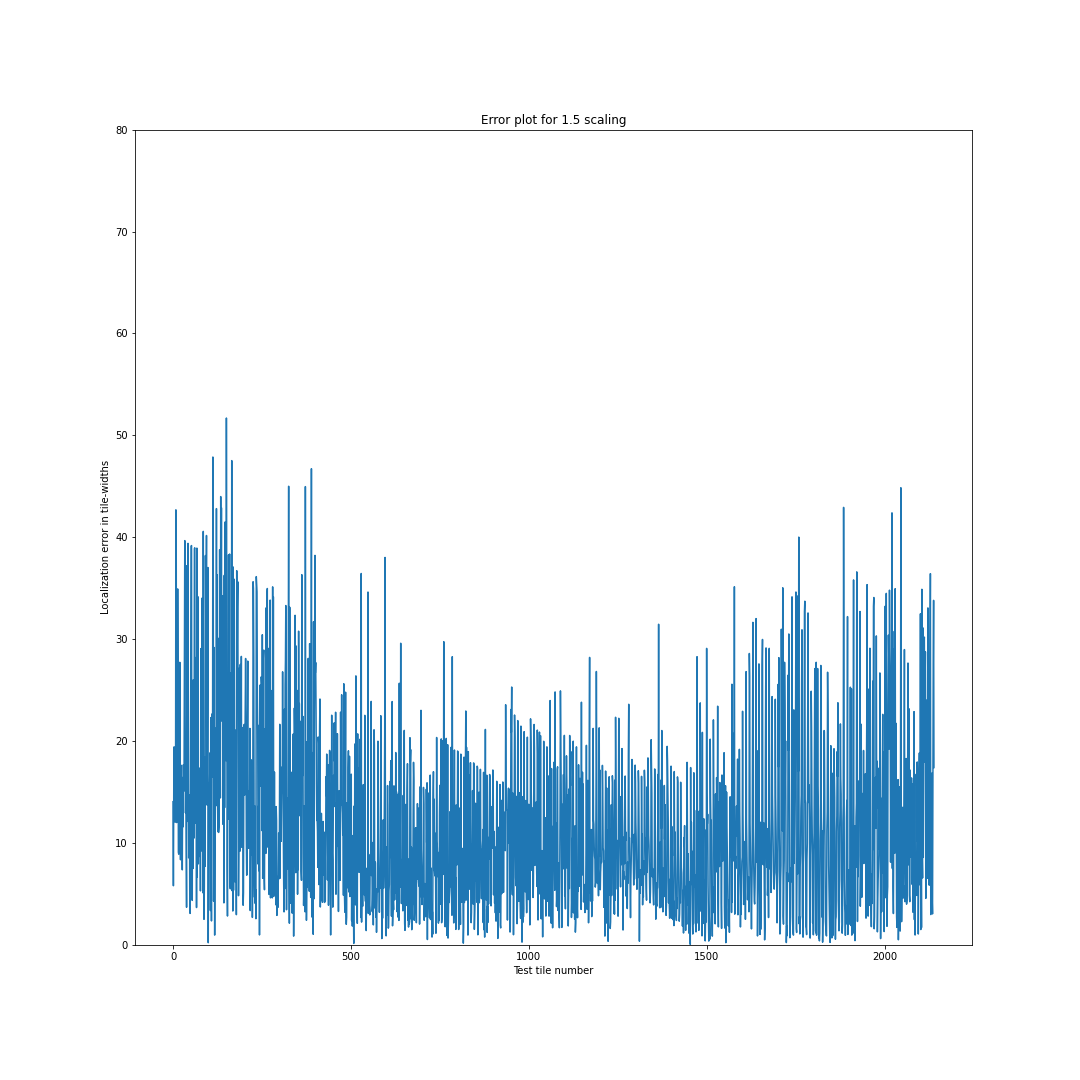
\includegraphics[width = 1.5in]{figures/thesis/plt_folder/scale_error_1.5}}&
		\subfloat[1.5 scaling error distribution]{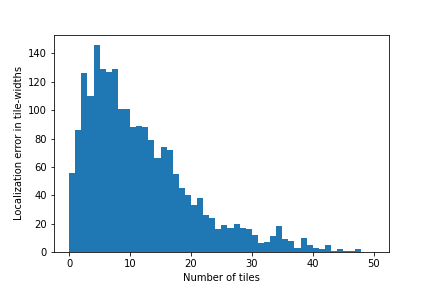
\includegraphics[width = 1.5in]{figures/thesis/plt_folder/scale_hist_1.5}}\\
		\subfloat[1.9 scaling]{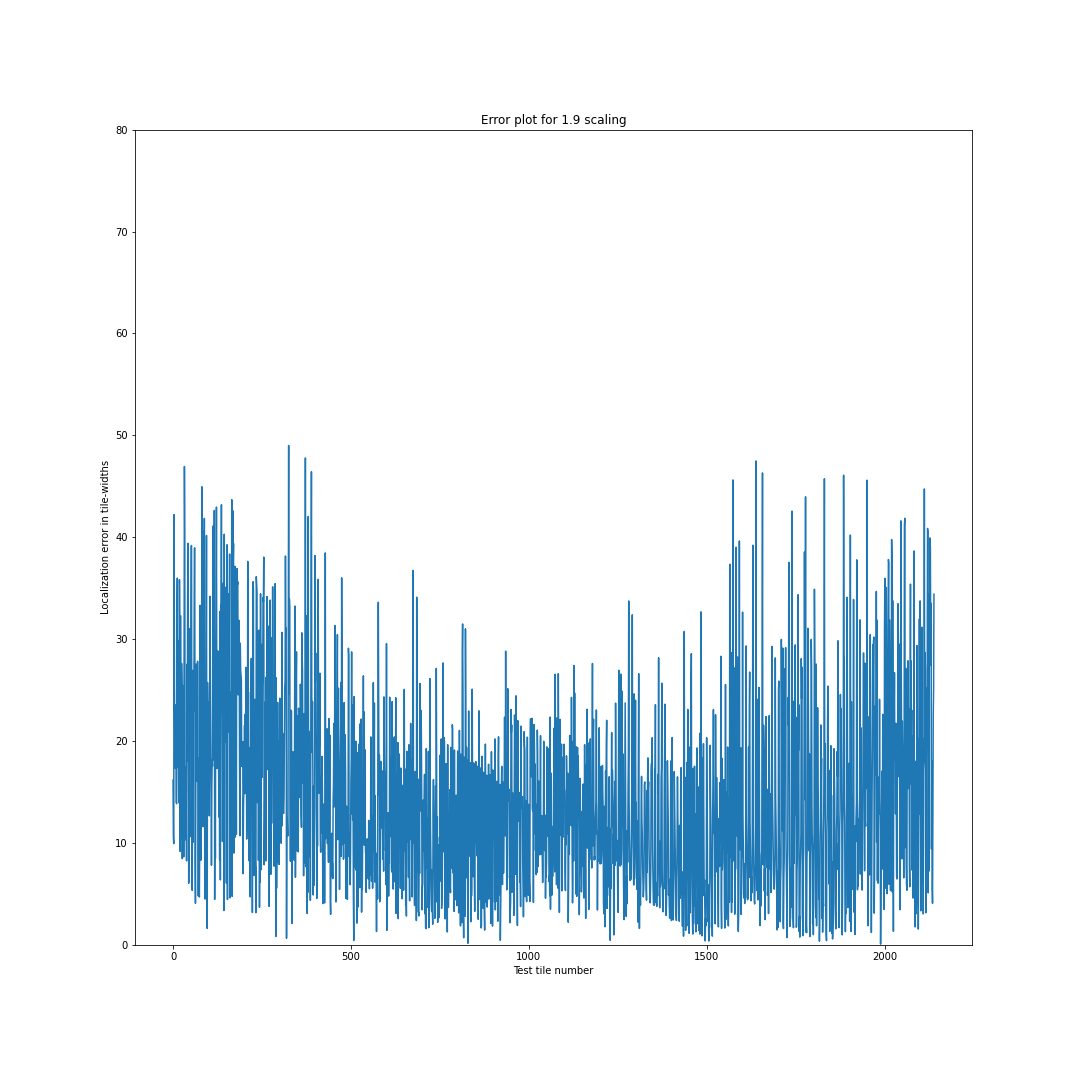
\includegraphics[width = 1.5in]{figures/thesis/plt_folder/scale_error_1.9}} &
		\subfloat[1.9 scaling error distribution]{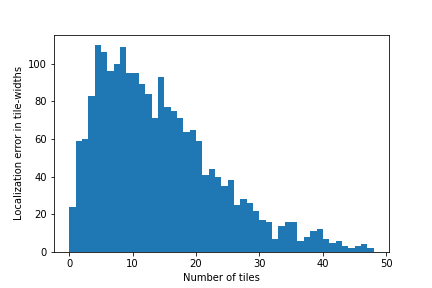
\includegraphics[width = 1.5in]{figures/thesis/plt_folder/scale_hist_1.9}}\\
		\subfloat[2.3 scaling]{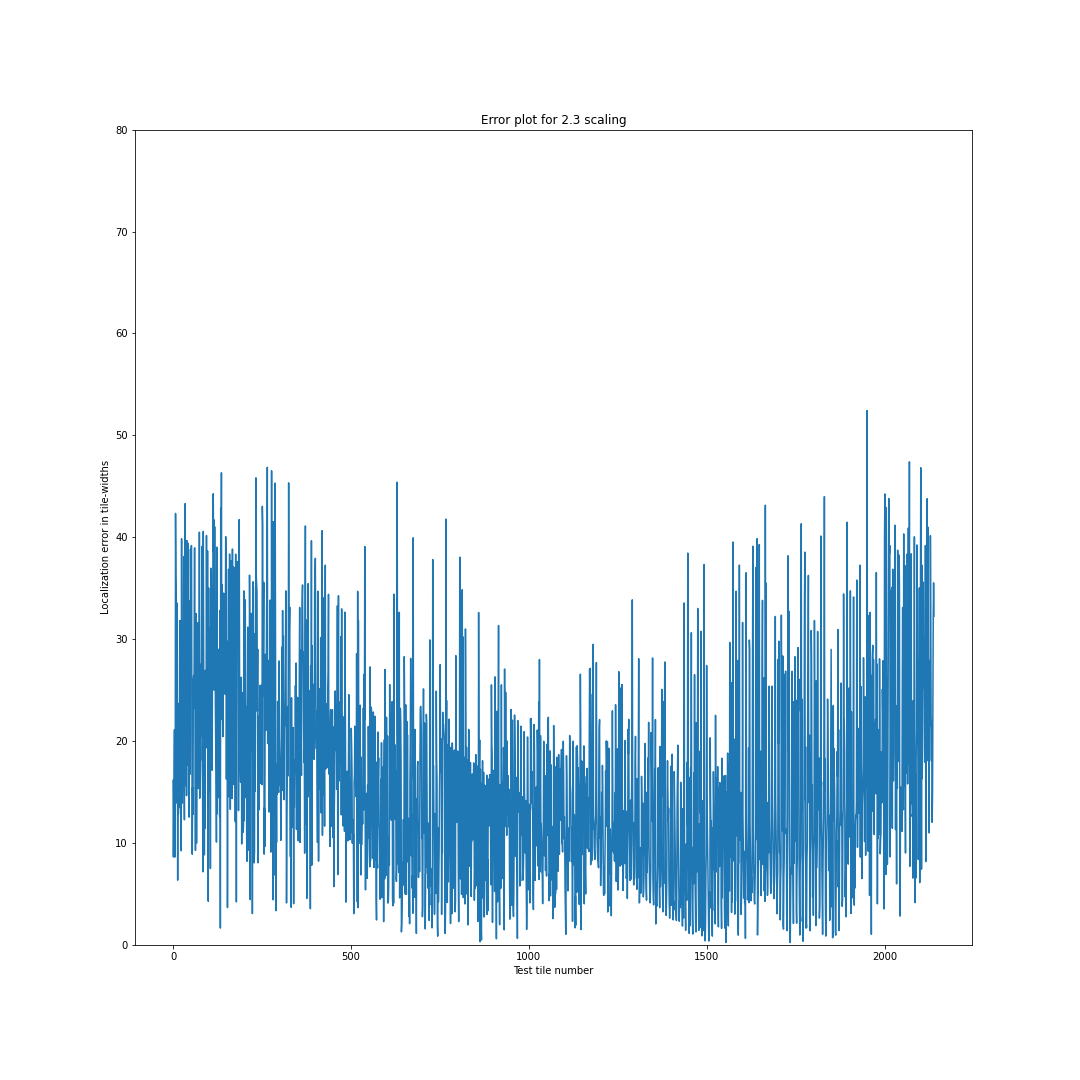
\includegraphics[width = 1.5in]{figures/thesis/plt_folder/scale_error_2.3}} &
		\subfloat[2.3 scaling error distribution]{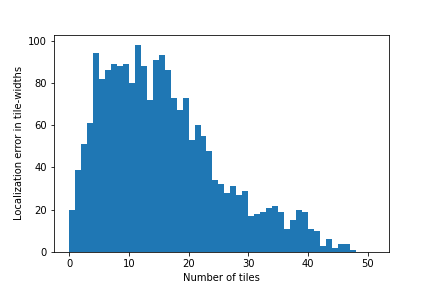
\includegraphics[width = 1.5in]{figures/thesis/plt_folder/scale_hist_2.3}}\\
		\subfloat[2.7 scaling]{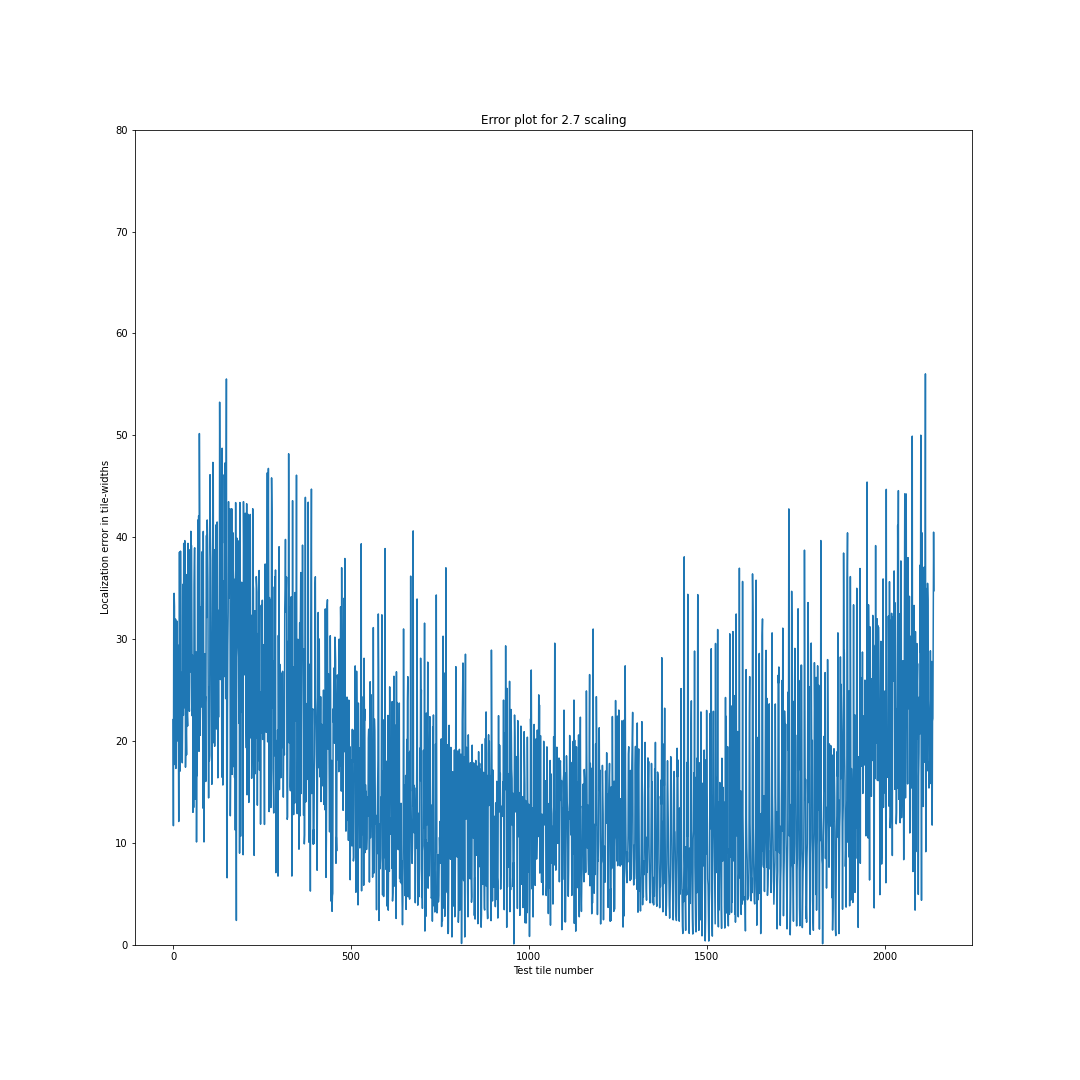
\includegraphics[width = 1.5in]{figures/thesis/plt_folder/scale_error_2.7}}&
		\subfloat[2.7 scaling error distribution]{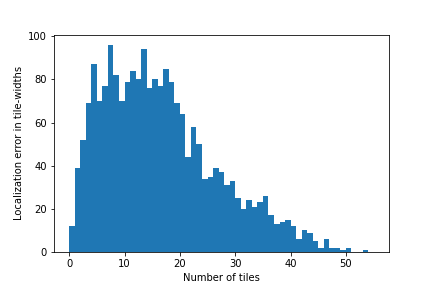
\includegraphics[width = 1.5in]{figures/thesis/plt_folder/scale_hist_2.7}}
	\end{longtable}
	\caption{Effect of scaling on localization. We check the error for scaling steps of 0.4 scale increments for the entire dataset, and show that as deviations from the actual orientation yields higher errors.}
\end{figure}

\subsection{Evaluation on query tiles constructed from the actual Oxford Sequence}

As we have stated, we evaluate our method on the Oxford Robotcar Dataset (\textcite{newman2017}). All the sequences of the RobotCar dataset are runs on a fixed route in different times and conditions. We choose the sequence \textbf{2015-03-17-11-08-44} for our evaluations.

\subsubsection{Evaluating for the Oxford RobotCar sequence}
For evaluation, we choose those locations in our oxford sequence that are as close as possible to those tiles in our training sequence that have a low localization error (within 1 tile distance). This way, we can make a fair evaluation in the sense that the locations we are testing from the Oxford Dataset are known to have done well when represented with standard OSM tiles.

Even though our Oxford Robotcar query locations will not overlap exactly with their corresponding OSM tiles of the training dataset, we can still make an evaluation of localization based on how close we can get to our representation to OSM tile.

\myfig{thesis/oxford_dataset_traj.png}%% filename
{scale=0.25}%%oxford_dataset_traj.png width/height
{Trajectory of Oxford Dataset drive}%% caption
{Oxford dataset trajectory}%% optional (short) caption for list of figures
{Ev1.7}

We have sampled query locations almost uniformly from the oxford trajectory. We choose those locations with distinct building geometry, rejecting empty of nearly empty locations around a candidate query location.

\pagebreak
We observe from the below figure that we have sampled locations uniformly from the original oxford driving trajectory. 

\myfig{thesis/query_dataset_traj.png}%% filename
{scale=0.3}%%oxford_dataset_traj.png width/height
{Query locations for evaluation}%% caption
{Query locations}%% optional (short) caption for list of figures
{Ev1.8}

As we have described in our methodology section, we create query map tiles at the locations shown above and evaluate how well the network localizes our query tiles at the locations sampled from the oxford robotcar trajectory. 

We show below statistics of our system's performance:

\myfig{thesis/error_gps_query.png}%% filename
{scale=0.5}%%oxford_dataset_traj.png width/height
{Blue - GPS positions of ground truth. Red - GPS positions of prediction}%% caption
{Query prediction GPS}%% optional (short) caption for list of figures
{Ev1.9}

\myfig{thesis/pred_1.png}%% filename
{scale=0.3}%%oxford_dataset_traj.png width/height
{Blue - GPS positions of ground truth. Red - GPS positions of prediction. Locations with errors rounded to 1 Tile Width}%% caption
{Query prediction less than 1 Tile Width}%% optional (short) caption for list of figures
{Ev2.0}

\myfig{thesis/pred_2.png}%% filename
{scale=0.3}%%oxford_dataset_traj.png width/height
{Blue - GPS positions of ground truth. Red - GPS positions of prediction.Locations with errors rounded to 2 Tile Width}%% caption
{Query prediction less than 2 Tile Width}%% optional (short) caption for list of figures
{Ev2.1}

\myfig{thesis/pred_3.png}%% filename
{scale=0.3}%%oxford_dataset_traj.png width/height
{Blue - GPS positions of ground truth. Red - GPS positions of prediction. Locations with errors rounded to 3 Tile Width}%% caption
{Query prediction less than 3 Tile Width}%% optional (short) caption for list of figures
{Ev2.2}

\myfig{thesis/pred_4.png}%% filename
{scale=0.3}%%oxford_dataset_traj.png width/height
{Blue - GPS positions of ground truth. Red - GPS positions of prediction. Locations with errors rounded to 4 Tile Width}%% caption
{Query prediction less than 4 Tile Width}%% optional (short) caption for list of figures
{Ev2.3}

\myfig{thesis/pred_5.png}%% filename
{scale=0.3}%%oxford_dataset_traj.png width/height
{Blue - GPS positions of ground truth. Red - GPS positions of prediction. Locations with errors rounded to 5 Tile Width}%% caption
{Query prediction less than 5 Tile Width}%% optional (short) caption for list of figures
{Ev2.4}

\myfig{thesis/pred_6.png}%% filename
{scale=0.3}%%oxford_dataset_traj.png width/height
{Blue - GPS positions of ground truth. Red - GPS positions of prediction. Locations with errors rounded to 6 Tile Width}%% caption
{Query prediction less than 6 Tile Width}%% optional (short) caption for list of figures
{Ev2.5}

\myfig{thesis/error_hist_query.png}%% filename
{scale=0.5}%%oxford_dataset_traj.png width/height
{Localization error distribution over 237 locations in Oxford Trajectory}%% caption
{Query prediction error distribution}%% optional (short) caption for list of figures
{Ev2.6}

\myfig{thesis/error_graph_query.png}%% filename
{scale=0.2}%%oxford_dataset_traj.png width/height
{Error plot in tile units over the 237 query locations}%% caption
{Query prediction error plot}%% optional (short) caption for list of figures
{Ev2.6}

\pagebreak
We observe that the predictions are within 6 tile widths of the ground truth (this translates to approximately 600 meters). However, it has to be noted that we are able to narrow down the location to within a 6 tile radius (a search space of at most 91 tiles), given that the total search space is approximately 2500 tiles. 

\subsubsection{A qualitative evaluation of the results}
We display here a set of (constructed tile, predicted tile) pairs to get a sense of how exactly the MapNet pose regressor behaves in this setting.

\begin{figure}
	\begin{longtable}{cc}
		\centering
		\subfloat{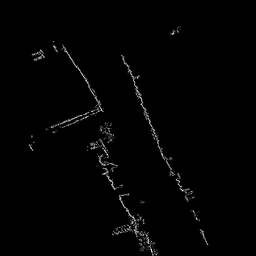
\includegraphics[width = 1.5in]{figures/thesis/evals/1.0/1_gt.png}}&
		\subfloat{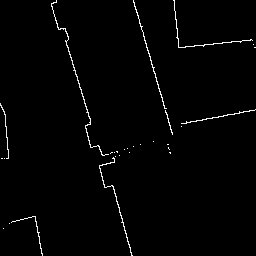
\includegraphics[width = 1.5in]{figures/thesis/evals/1.0/1_pred.png}}\\
		\subfloat{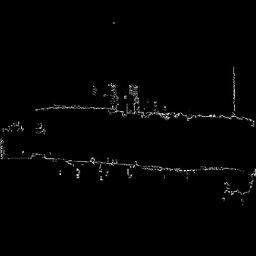
\includegraphics[width = 1.5in]{figures/thesis/evals/1.0/2_gt.png}} &
		\subfloat{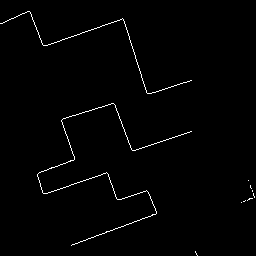
\includegraphics[width = 1.5in]{figures/thesis/evals/1.0/2_pred.png}}\\
		\subfloat{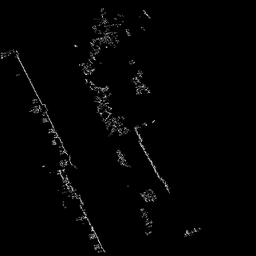
\includegraphics[width = 1.5in]{figures/thesis/evals/1.0/3_gt.png}} &
		\subfloat{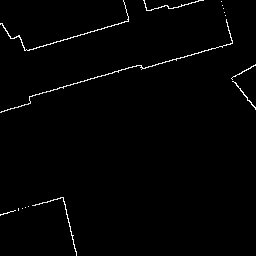
\includegraphics[width = 1.5in]{figures/thesis/evals/1.0/3_pred.png}}\\
		\subfloat{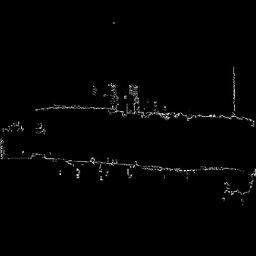
\includegraphics[width = 1.5in]{figures/thesis/evals/1.0/4_gt.png}}&
		\subfloat{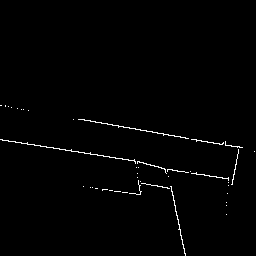
\includegraphics[width = 1.5in]{figures/thesis/evals/1.0/4_pred.png}}\\
	\end{longtable}
\end{figure}

\begin{figure}
	\begin{longtable}{cc}
		\subfloat{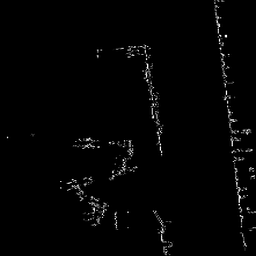
\includegraphics[width = 1.5in]{figures/thesis/evals/1.0/5_gt.png}}&
		\subfloat{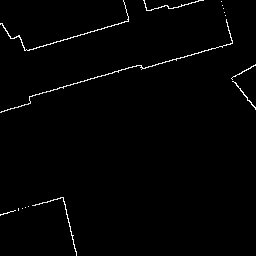
\includegraphics[width = 1.5in]{figures/thesis/evals/1.0/5_pred.png}}
	\end{longtable}
	\caption{Left - query tile, Right - Predicted tile on raster. Examples with Localization errors less than 1 Tile Width}
\end{figure}

\pagebreak
We note that the prediction manages to find structure quite similar to the kind of structure present in the query tiles. Note that as long as noise conforms somewhat to the true contours of the buildings around them, we get a good prediction that is close to the location of the query tile.

\begin{figure}
	\begin{longtable}{cc}
		\centering
		\subfloat{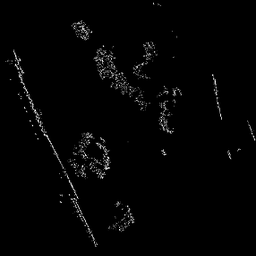
\includegraphics[width = 1.5in]{figures/thesis/evals/2.0/1_gt.png}}&
		\subfloat{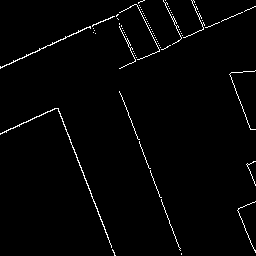
\includegraphics[width = 1.5in]{figures/thesis/evals/2.0/1_pred.png}}\\
		\subfloat{\includegraphics[width = 1.5in]{figures/thesis/evals/2.0/2_gt.png}} &
		\subfloat{\includegraphics[width = 1.5in]{figures/thesis/evals/2.0/2_pred.png}}\\
		\subfloat{\includegraphics[width = 1.5in]{figures/thesis/evals/2.0/3_gt.png}} &
		\subfloat{\includegraphics[width = 1.5in]{figures/thesis/evals/2.0/3_pred.png}}\\
	    \subfloat{\includegraphics[width = 1.5in]{figures/thesis/evals/2.0/4_gt.png}}&
		\subfloat{\includegraphics[width = 1.5in]{figures/thesis/evals/2.0/4_pred.png}}\\
	\end{longtable}
\end{figure}

\begin{figure}
	\begin{longtable}{cc}
		\subfloat{\includegraphics[width = 1.5in]{figures/thesis/evals/2.0/5_gt.png}}&
		\subfloat{\includegraphics[width = 1.5in]{figures/thesis/evals/2.0/5_pred.png}}
	\end{longtable}
	\caption{Left - query tile, Right - Predicted tile on raster. Examples with Localization errors less than 2 Tile Width}
\end{figure}

\pagebreak
Looking at a few tiles with localization error of less than 2 tile widths, we observe that the network predicts tiles with similar structures which conform well to the original structure but are led astray by noise. 

\begin{figure}
	\begin{longtable}{cc}
		\centering
		\subfloat{\includegraphics[width = 1.5in]{figures/thesis/evals/3.0/1_gt.png}}&
		\subfloat{\includegraphics[width = 1.5in]{figures/thesis/evals/3.0/1_pred.png}}\\
		\subfloat{\includegraphics[width = 1.5in]{figures/thesis/evals/3.0/2_gt.png}} &
		\subfloat{\includegraphics[width = 1.5in]{figures/thesis/evals/3.0/2_pred.png}}\\
		\subfloat{\includegraphics[width = 1.5in]{figures/thesis/evals/3.0/3_gt.png}} &
		\subfloat{\includegraphics[width = 1.5in]{figures/thesis/evals/3.0/3_pred.png}}\\
		\subfloat{\includegraphics[width = 1.5in]{figures/thesis/evals/3.0/4_gt.png}}&
		\subfloat{\includegraphics[width = 1.5in]{figures/thesis/evals/3.0/4_pred.png}}
	\end{longtable}
\end{figure}

\begin{figure}
	\begin{longtable}{cc}
		\subfloat{\includegraphics[width = 1.5in]{figures/thesis/evals/3.0/5_gt.png}}&
		\subfloat{\includegraphics[width = 1.5in]{figures/thesis/evals/3.0/5_pred.png}}
	\end{longtable}
	\caption{Left - query tile, Right - Predicted tile on raster. Examples with Localization errors less than 3 Tile Width}
\end{figure}

\pagebreak
We still observe that the predictions are structurally similar to query tiles, but cannot be on point thanks to the noise contributed by trees segmented as buildings. 


\begin{figure}
	\begin{longtable}{cc}
		\centering
		\subfloat{\includegraphics[width = 1.5in]{figures/thesis/evals/4.0/1_gt.png}}&
		\subfloat{\includegraphics[width = 1.5in]{figures/thesis/evals/4.0/1_pred.png}}\\
		\subfloat{\includegraphics[width = 1.5in]{figures/thesis/evals/4.0/2_gt.png}} &
		\subfloat{\includegraphics[width = 1.5in]{figures/thesis/evals/4.0/2_pred.png}}\\
		\subfloat{\includegraphics[width = 1.5in]{figures/thesis/evals/4.0/3_gt.png}} &
		\subfloat{\includegraphics[width = 1.5in]{figures/thesis/evals/4.0/3_pred.png}}\\
		\subfloat{\includegraphics[width = 1.5in]{figures/thesis/evals/4.0/4_gt.png}}&
		\subfloat{\includegraphics[width = 1.5in]{figures/thesis/evals/4.0/4_pred.png}}
	\end{longtable}
\end{figure}

\begin{figure}
	\begin{longtable}{cc}
		\subfloat{\includegraphics[width = 1.5in]{figures/thesis/evals/4.0/5_gt.png}}&
		\subfloat{\includegraphics[width = 1.5in]{figures/thesis/evals/4.0/5_pred.png}}
	\end{longtable}
	\caption{Left - query tile, Right - Predicted tile on raster. Examples with Localization errors less than 4 Tile Width}
\end{figure}

\pagebreak
Structural similarity is still observable in the predictions, but noise confuses the network because it doesn't conform to the true building outline to give a good enough prediction. 

\begin{figure}
	\begin{longtable}{cc}
		\centering
		\subfloat{\includegraphics[width = 1.5in]{figures/thesis/evals/5.0/1_gt.png}}&
		\subfloat{\includegraphics[width = 1.5in]{figures/thesis/evals/5.0/1_pred.png}}\\
		\subfloat{\includegraphics[width = 1.5in]{figures/thesis/evals/5.0/2_gt.png}} &
		\subfloat{\includegraphics[width = 1.5in]{figures/thesis/evals/5.0/2_pred.png}}\\
		\subfloat{\includegraphics[width = 1.5in]{figures/thesis/evals/5.0/3_gt.png}} &
		\subfloat{\includegraphics[width = 1.5in]{figures/thesis/evals/5.0/3_pred.png}}\\
		\subfloat{\includegraphics[width = 1.5in]{figures/thesis/evals/5.0/4_gt.png}}&
		\subfloat{\includegraphics[width = 1.5in]{figures/thesis/evals/5.0/4_pred.png}}
	\end{longtable}
\end{figure}

\begin{figure}
	\begin{longtable}{cc}
		\subfloat{\includegraphics[width = 1.5in]{figures/thesis/evals/5.0/5_gt.png}}&
		\subfloat{\includegraphics[width = 1.5in]{figures/thesis/evals/5.0/5_pred.png}}
	\end{longtable}
	\caption{Left - query tile, Right - Predicted tile on raster. Examples with Localization errors less than 5 Tile Width}
\end{figure}

\pagebreak
Structural similarity is still observable in the predictions, but noise confuses the network because it doesn't conform to the true building outline to give a good enough prediction. 

\begin{figure}
	\begin{longtable}{cc}
		\centering
		\subfloat{\includegraphics[width = 1.5in]{figures/thesis/evals/6.0/1_gt.png}}&
		\subfloat{\includegraphics[width = 1.5in]{figures/thesis/evals/6.0/1_pred.png}}\\
		\subfloat{\includegraphics[width = 1.5in]{figures/thesis/evals/6.0/2_gt.png}} &
		\subfloat{\includegraphics[width = 1.5in]{figures/thesis/evals/6.0/2_pred.png}}\\
		\subfloat{\includegraphics[width = 1.5in]{figures/thesis/evals/6.0/3_gt.png}} &
		\subfloat{\includegraphics[width = 1.5in]{figures/thesis/evals/6.0/3_pred.png}}\\
		\subfloat{\includegraphics[width = 1.5in]{figures/thesis/evals/6.0/4_gt.png}}&
		\subfloat{\includegraphics[width = 1.5in]{figures/thesis/evals/6.0/4_pred.png}}
	\end{longtable}
\end{figure}

\begin{figure}
	\begin{longtable}{cc}
		\subfloat{\includegraphics[width = 1.5in]{figures/thesis/evals/6.0/5_gt.png}}&
		\subfloat{\includegraphics[width = 1.5in]{figures/thesis/evals/6.0/5_pred.png}}
	\end{longtable}
	\caption{Left - query tile, Right - Predicted tile on raster. Examples with Localization errors less than 6 Tile Width}
\end{figure}

\pagebreak
Structural similarity is still observable in the predictions, but noise confuses the network because it doesn't conform to the true building outline to give a good enough prediction. 




